\subparagraph{Задание 4.4}

\textbf{Условие}:
В любой инструкции с двумя операндами удалить один операнд и проассемблировать программу с получением файла листинга. Какие выходные файлы создаются в этом случае? Что добавляется в листинге? Привести результаты наблюдений в отчете и объяснить их.

\textbf{Решение}:

\begin{lstlisting}[language=Terminal]
$ C:\tasm\tasm.exe Lab2.asm,,Lab2-1.lst
\end{lstlisting}

\begin{lstlisting}[language=Out]
Turbo Assembler  Version 2.0  Copyright (c) 1988, 1990 Borland International

Assembling file:   Lab2.asm
Error messages:    None
Warning messages:  None
Passes:            1
Remaining memory:  469k
\end{lstlisting}

\textbf{Создался} файл листинга \textbf{LAB2-1.LST} и объктный файл \textbf{LAB2.OBJ}.

\begin{lstlisting}[language=Terminal]
$ C:\tasm\tasm.exe Lab2.asm,,Lab2-2.lst
\end{lstlisting}

\begin{lstlisting}[language=Out]
Turbo Assembler  Version 2.0  Copyright (c) 1988, 1990 Borland International

Assembling file:   Lab2.asm
**Error** Lab2.asm(11) Too few operands to instruction
Error messages:    1
Warning messages:  None
Passes:            1
Remaining memory:  469k
\end{lstlisting}

\textbf{Создался} только файл листинга \textbf{LAB2-2.LST} (объектный файл \textbf{LAB2.OBJ не создался}).

\begin{figure}[h]
    \centering
    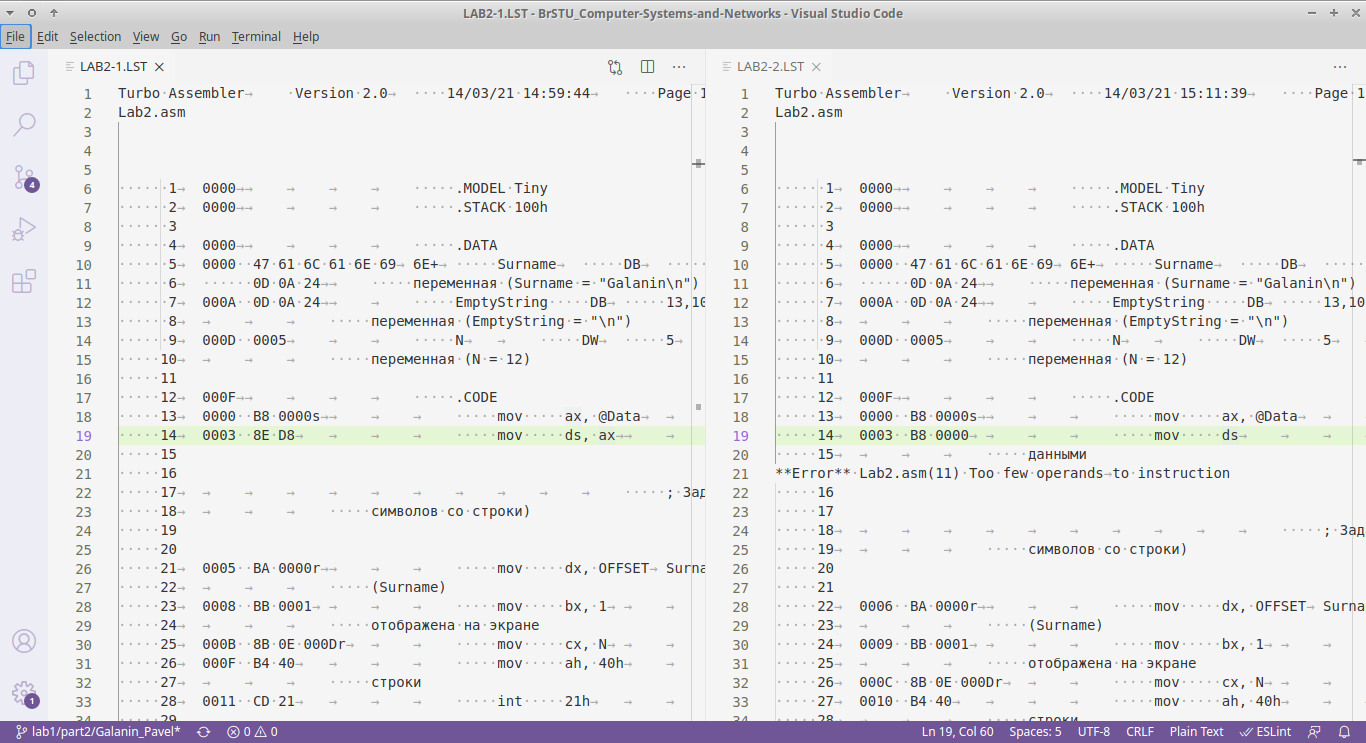
\includegraphics[width=18cm]
        {../_INCLUDES/task-4-4/lst1-and-lst2.png}
    \caption{Сравнение LAB2-1.LST и LAB2-2.LST в VS Code}
\end{figure}
